\documentclass[12pt]{article}

\usepackage[margin=1in]{geometry}
\usepackage{amsmath}
\usepackage{amssymb}
\usepackage{graphicx}
\usepackage{booktabs}
\usepackage{hyperref}
\usepackage[capitalise]{cleveref}
\usepackage{microtype}
\usepackage{fancyvrb}
\usepackage{parskip}

\usepackage{tikz}
\usetikzlibrary{arrows.meta, positioning, shapes.geometric, calc, fit}

\usepackage{array}
\usepackage{tabularx}
\newcolumntype{L}[1]{>{\raggedright\arraybackslash}p{#1}}
\newcolumntype{C}[1]{>{\centering\arraybackslash}p{#1}}

% Figures live in ./images (p_step.pdf is generated by code/gen_figures_intro_pcontrol.m)
\graphicspath{{./}}

% Draft review flag: \verify{note} renders an inline orange callout.
% Redefine to \newcommand{\verify}[1]{} to suppress all flags in a clean build.
\newcommand{\verify}[1]{\textcolor{orange}{\textbf{[?~#1]}}}

\newcommand{\figplaceholder}[2][3in]{%
  \begin{center}
  \fbox{\parbox{#1}{\centering\vspace{0.5in}\textit{[Figure: #2]}\vspace{0.5in}}}
  \end{center}
}

\hypersetup{
  pdftitle  = {USV Control Case Study, Part 1: Introduction and PID feedback control},
  pdfauthor = {Brian Bingham},
}

\begin{document}

\begin{center}
   \setlength{\parskip}{0pt}
  {\LARGE USV Control Case Study\par}
  {\Large Part 1: Introduction and proportional control\par}
  \vspace{0.8em}
  Brian Bingham \quad\textbar\quad Fall 2026
\end{center}
\tableofcontents


% ===========================================================================
\section{Introduction}
\label{sec:intro}
% ===========================================================================

This is the first part of a short series on feedback control, from design to implementation.  Rather than develop the ideas in the abstract, we use the USV from our labs as a case study: a specific example of general principles that apply to most controlled systems.

 We have driven the USV and identified models of its surge and yaw dynamics, so we already have some intuition for how the plant behaves: how responds to throttle commands and rudder deflection.  The intent is that this intuition guides our understanding the various aspects of  the controller implementation.

The USV problems represent the most common class of control problems, \emph{setpoint tracking}.  We command a desired value of the output (the setpoint), such as a speed or a heading, and want the output to reach that value quickly, without excessive overshoot, and then hold it despite disturbances like wind and current.  The setpoint changes  by operator command or when the vehicle reaches a waypoint.  The step response is therefore the natural measure of performance which is categorized as transient performance (rise time, overshoot, settling time, etc.) and steady-state error.

\subsection*{USV Scenario}

We will use two running examples drawn directly from
the USV labs.

\begin{figure}[htbp]
\centering
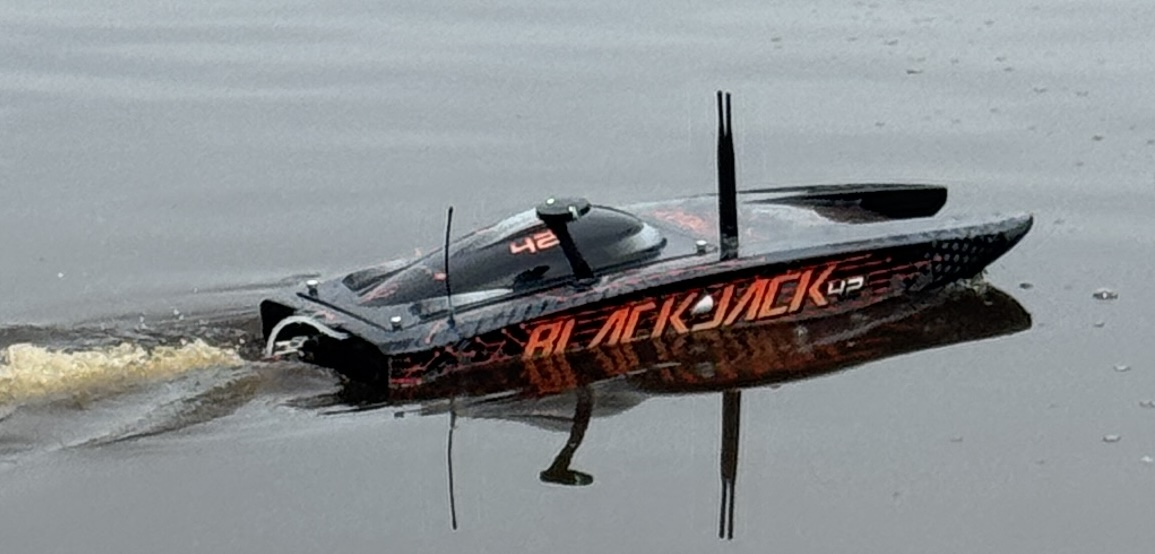
\includegraphics[width=0.7\textwidth]{images/usv_nps.jpg}
\caption{The USV used in the lab.}
\label{fig:usv}
\end{figure}

\textbf{Surge (speed) control.}
The USV's forward speed response to throttle can be approximated by a
first-order transfer function.  The objective is to hold a desired speed in the presence of disturbances like current and wind --- it is a
\emph{constant-setpoint tracking problem}, the simplest and most common control
scenario.

\textbf{Heading control.}
The USV's yaw-rate response to rudder is also first-order, but the performance
metric we care about is \emph{heading} (yaw angle), which is the integral of
yaw rate.  This mismatch between the plant output and the performance metric
turns out to be the key motivation for \emph{cascade control}: an inner loop
that regulates yaw rate quickly, wrapped inside an outer loop that uses that
fast inner response to achieve precise heading.  This is also the architecture
used by ArduRover.


% ===========================================================================
\section{The PID Feedback Controller}
\label{sec:pid}
% ===========================================================================

\subsection{Conceptual Overview}

The PID controller computes a corrective input from three components of the
error $e(t) = r(t) - y(t)$, where $r(t)$ is the reference (also called
the \emph{command} or \emph{setpoint}) and $y(t)$ is the measured output.

\begin{description}
  \item[Proportional ($K_P$)] React to the current error.  If the vessel is
    2\,m/s below target speed, apply a corrective throttle proportional to
    that gap.  Larger error, larger correction.
  \item[Integral ($K_I$)] Adapt to the history of error.  As long as any error persists, however small, the integrator keeps growing (winding up), so the controller adapts to what it does not know in advance.  Holding a cruise speed takes a constant thrust to overcome hull drag, and the integrator finds that throttle level without a model of the drag.  Similarly, unmodeled environmental factors (wind, water currents) affects the vessel performance, and the integrator builds up the extra throttle needed to cancel it.
  \item[Derivative ($K_D$)] Anticipate the future error.  If the speed error is
    shrinking rapidly, the vessel is closing in on its target, the
    derivative term begins reducing the throttle command before the speed
    overshoots.
\end{description}

A useful analogy is a driver trying to hold a fixed highway speed.  The P term
is how firmly they press the accelerator in proportion to how far off-speed they are.
The I term represents what the driver has learned about the road grade and
headwind, accumulated experience that shows up as a steady baseline pressure
on the pedal.  The D term is the instinctive easing-off as the speedometer rapidly approaches the target speed. 

\subsection{Transfer Function Form}

Expressed in the time-domain, the PID control law is:
\begin{equation}
  u(t) = K_P\, e(t) \;+\; K_I \int_0^t e(\tau)\,d\tau \;+\; K_D\, \dot{e}(t)
  \label{eq:pid_time}
\end{equation}
where $u(t)$ is the control input (USV throttle command) and $e(t)$ is the error signal (difference between desired and actual speed).

Expressed in the Laplace domain, the PID control law gives the controller transfer function:
\begin{equation}
  C(s) = \frac{U(s)}{E(s)} = K_P + \frac{K_I}{s} + K_D s = \frac{K_D s^2 + K_P s + K_I}{s}
  \label{eq:pid_tf}
\end{equation}

Two features are worth noting.  First, there is one pole at $s = 0$: the
integrator.  We will see in the section on integral action exactly why this eliminates
steady-state error.  Second, there are two zeros, at the roots of
$K_D s^2 + K_P s + K_I = 0$.  The designer places these anywhere in the
complex plane by choosing $K_P$, $K_I$, and $K_D$, giving the designer significant freedom to
shape the closed-loop response.

Note that $K_D s$ grows without bound as $s \to \infty$.  This means the ideal
PID transfer function is \emph{improper} and cannot be implemented exactly in
hardware or software.  In practice, the D term always includes a high-frequency
limit; we will address this when we cover practical modifications to PID.

\subsection{Closed-Loop Transfer Function}

To be explicit in our notation, we use the general unity feedback architecture as shown in \cref{fig:unity_feedback}.  We'll customize this for the USV speed and heading control problem in the following sections.

\begin{figure}[htbp]
\centering
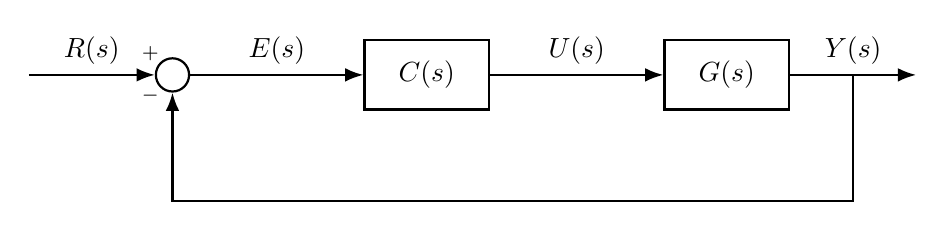
\begin{tikzpicture}[
  >=Latex, thick,
  block/.style = {draw, rectangle, minimum height=2.5em, minimum width=4.5em},
  sum/.style   = {draw, circle, inner sep=0pt, minimum size=1.2em},
]
  \node[coordinate]                   (rin)  {};
  \node[sum,   right=1.6cm of rin]    (sum)  {};
  \node[block, right=2.2cm of sum]    (C)    {$C(s)$};
  \node[block, right=2.2cm of C]      (G)    {$G(s)$};
  \node[coordinate, right=1.6cm of G] (yout) {};

  % Signs at summing junction
  \node[font=\scriptsize, inner sep=0pt, anchor=south east] at (sum.north west) {$+$};
  \node[font=\scriptsize, inner sep=0pt, anchor=north east] at (sum.south west) {$-$};

  % Forward path
  \draw[->] (rin)  -- node[above]{$R(s)$}  (sum);
  \draw[->] (sum)  -- node[above]{$E(s)$}  (C);
  \draw[->] (C)    -- node[above]{$U(s)$}  (G);
  \draw[->] (G)    -- node[above]{$Y(s)$}  (yout);

  % Feedback path: down from midpoint of output wire, left, up into sum
  \coordinate (fbk) at ($(G.east)!0.5!(yout)$);
  \draw[->] (fbk) -- ++(0,-1.6) -| (sum.south);
\end{tikzpicture}
\caption{Standard unity-feedback control loop.}
\label{fig:unity_feedback}
\end{figure}

The closed-loop transfer function is:
\begin{equation}
  T(s) = \frac{Y(s)}{R(s)} = \frac{C(s)G(s)}{1 + C(s)G(s)}
  \label{eq:cltf}
\end{equation}

% ===========================================================================
\section{Proportional Control of Speed as a First-Order Plant}
\label{sec:pcontrol}
% ===========================================================================

\subsection{The USV Surge Model}

We've seen that the USV's surge (forward speed, $v_x$) dynamics can be approximated as a first-order system.

Linear analysis of the surge dynamics (forward speed vs.\ throttle) yields a
first-order transfer function:
\begin{equation}
  G_{v_x}(s) = \frac{Y(s)}{U(s)} = \frac{K_{v_x}}{\tau_{v_x} s + 1}
  \label{eq:surge_plant}
\end{equation}
where $K_{v_x}$, the DC gain, is the steady-state speed per unit throttle (m/s per unit effort)
and $\tau_{v_x}$ is the time constant set by the balance of inertia and drag.
Throttle is normalized to $\pm 1$, with $+1$ being full forward effort and
$-1$ full reverse.

\subsection{Closed-Loop with P Only}

Starting with the minimial viable controll law for speed regulation allows us to preserve some intuitive understanding of the system's behavior and keeps the analysis simple enough to derive closed-form expressions for the closed-loop response.    These models, like all models, are wrong, but they are useful for gaining insight into the system's behavior.

The control law is our PID controller from \cref{sec:pid}, where we neglect the integral and derivative terms, leaving only the proportional term:
\[
C(s) = \frac{U(s)}{E(s)} = \frac{\text{throttle effort}}{\text{speed error}} = K_P
\]

This is the simplest form of feedback control, where the control effort is directly proportional to the error, i.e, $U_\text{throttle effort} = K_P \, (E_\text{speed error})$ - the larger the error, the larger the control effort applied.

The closed-loop transfer function for P-only control, derived using the first-order plant model, is



With a pure proportional controller $C(s) = K_P$, the open-loop transfer
function is $C(s)G(s) = K_P K_{v_x}/(\tau_{v_x} s + 1)$.  Substituting into
\cref{eq:cltf}:
\begin{equation}
  T(s) = \frac{K_P K_{v_x}/(\tau_{v_x} s+1)}{1 + K_P K_{v_x}/(\tau_{v_x} s+1)}
          = \frac{K_P K_{v_x}}{\tau_{v_x} s + 1 + K_P K_{v_x}}
          = \frac{K_\infty}{\tau_\mathrm{cl}\,s + 1}.
  \label{eq:cl_p}
\end{equation}
We have written the closed-loop transfer function in the standard first-order form, with DC gain $K_\infty$ and closed-loop time constant $\tau_\mathrm{cl}$, where:
where:
\begin{equation}
  K_\infty = \frac{K_P K_{v_x}}{1 + K_P K_{v_x}}, \qquad
  \tau_\mathrm{cl} = \frac{\tau_{v_x}}{1 + K_P K_{v_x}}
  \label{eq:p_params}
\end{equation}

The closed-loop is still first-order, but compared to the open-loop plant, two things have
changed: 

\begin{enumerate}
\item The time constant is smaller (faster response) and decreases with increasing $K_P$
\item The DC gain is less than one and approaches one as $K_P$ increases.
\end{enumerate}


The DC gain of the closed-loop system, $K_\infty$ is less than one, which is the root of the problem.  For a unit step in
desired speed, the steady-state output is $K_\infty$, so the
\emph{steady-state error} is:
\begin{equation}
  e_{ss} = 1 - K_\infty = \frac{1}{1 + K_P K_{v_x}}
  \label{eq:p_error}
\end{equation}

\begin{figure}[htbp]
\centering
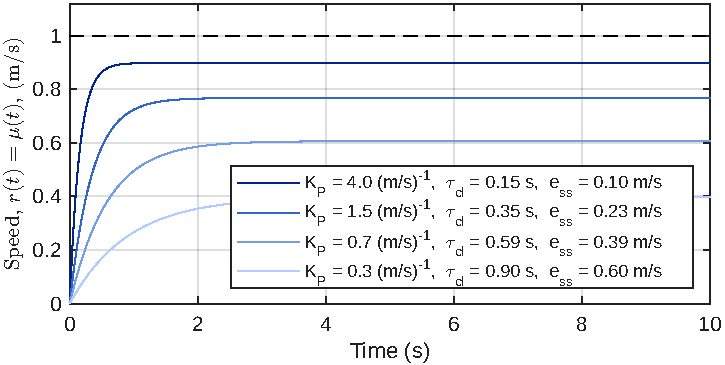
\includegraphics[width=\linewidth]{images/p_step.pdf}
\caption{Step response of the P-controlled surge plant for increasing
  proportional gain.  Higher gain improves transient speed and reduces error, but steady-state
  error persists regardless.}
\label{fig:p_step}
\end{figure}

\Cref{fig:p_step} shows graphically what \cref{eq:p_params,eq:p_error} show mathematically: two views of the same characteristics.  
\begin{enumerate}
\item As $K_P$ increases, the closed-loop time constant ($\tau_\mathrm{cl}$) shrinks and the response rises faster
\item As $K_P$ increases, the closed-loop DC gain ($K_\infty$) approaches one so $e_{ss}$ shrinks.  But for any finite $K_P$, $K_\infty < 1$ and the error never reaches zero.  (To eliminate it entirely, we need a different kind of controller action, integral action and/or feedforward.)
\item The form of the closed-loop transfer function remains first-order, even with proportional-only control.  The system does not become unstable as $K_P$ increases and there is never any oversoot; it simply responds faster and with reduced steady-state error.
\end{enumerate}


\end{document}
